\section{Électroaimant}
Le modèle utilisé pour caractériser l'électroaimant a été très simple.
Dans un premier lieu, nous avons approximé le coeur de fer rond par un transformateur conventionnel.
Aussi on s'est limité à l'expression de la force magnétomotrice (FMM) dans le coeur de fer. En effet, les trésors pèsent environ 27 g et les moyens dont on dispose peuvent générer des électroaimants
qui peuvent soulever des masses largement supérieures. Alors on a observé l'équation de la FMM.

\begin{equation}
FMM = NI
\end{equation}

Donc pour produire la FMM, on peut jouer sur le nombre de tours ou le courant qu'on peut injecter dans notre électroaimant.
Puisque notre électroaimant est alimenté par une banque de condensateur, il faut maximiser le nombre de tours pour générer la FMM nécessaire afin de limiter le courant pour lever le trésor.
Ainsi, on allonge le temps qu'on peut maintenir le trésor. Cependant, mettre un trop grand nombre de tours et la résistance va devenir trop élèvé et on ne sera plus en mesure de lever le trésor.
Pour déterminer, le calibre du fils et le nombre de tours, on a calculé dans le Excel, le nombre de tours maximal qu'on peut bobiner par chaque calibre et la résistance résultante.
On néglige le comportement dynamique de la bobine, car on est en quasi-statique/statique dans ce problème. Le résultat était du calibre 27 lequel on a bobiné environ 120 tours et on obtient
une résistance de $1.23 \Omega$. On peut maintenir le trésor pendant 3 minutes environ avec cet arrangement.

\subsection{Drive de l'électroaimant}

À cause que l'électroaimant va être drivé par un mosfet qui va fonctionner dans la zone de commutation, il faut mettre une diode de roue libre aux bornes de l'électroaimant.
On a choisi une diode Schottky à cause de sa grande vitesse de commutation.

  \begin{figure}[H]
    \label{Bobine}
    \centering
    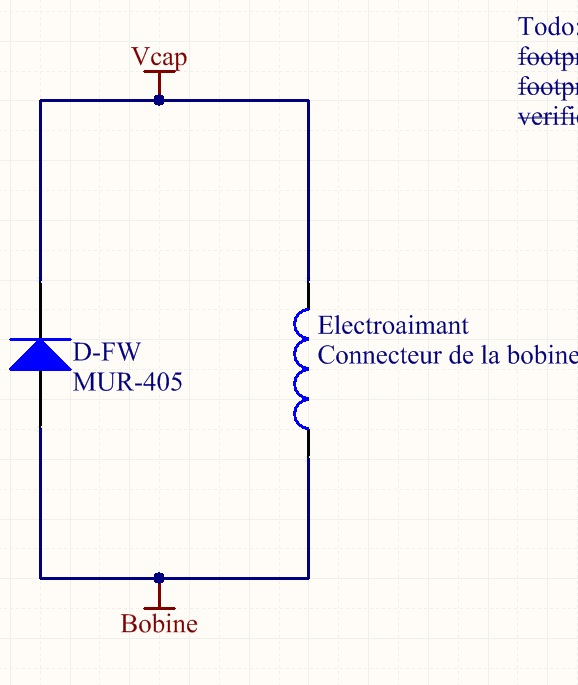
\includegraphics[scale=0.3]{resources/bobine.jpg}
    \caption{Bobine}
  \end{figure}

Afin de mettre du courant dans la bobine, on utilise un MOSFET N-MOS IRF540.
Le transistor est commandé par un PWM qui indique la commande de courant dans le transistor.
Cette solution a été la première penser à cause de sa très grande simplicité et cette solution a été retenue très rapidement à cause de son bon fonctionnement dans notre application.

  \begin{figure}[H]
    \label{drive}
    \centering
    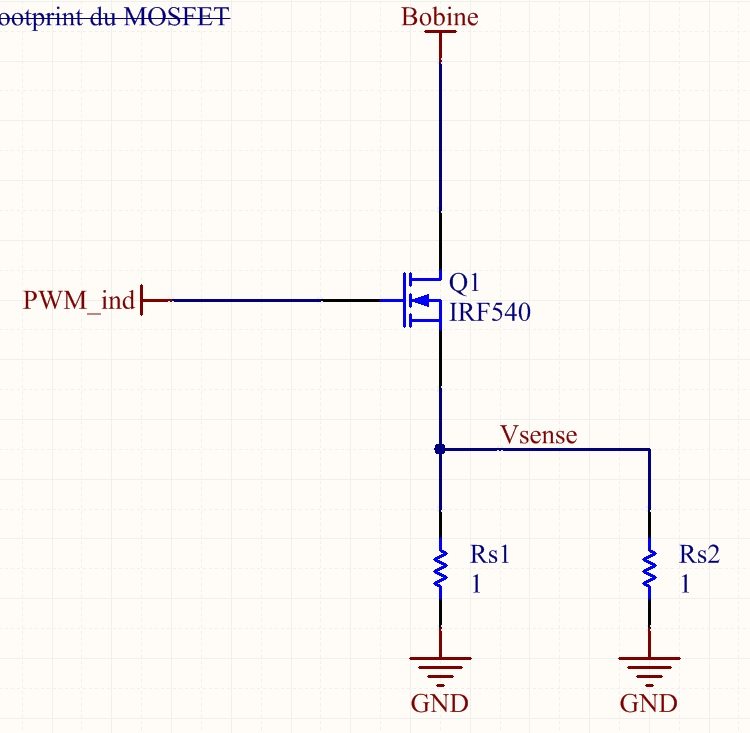
\includegraphics[scale=0.3]{resources/drivemosfet.jpg}
    \caption{Circuit de puissance de la bobine}
  \end{figure}

\subsection{Régulation de l'électroaimant}
Pour maintenir les trésors, il faut avoir un courant constant dans la bobine.
Pour ce faire, on avait deux solutions disponible: soit faire un asservissement analogique ou un asservissement numérique avec notre microcontrolleur.
L'avantage de l'asservissement numérique est qu'il coûte moins cher en pièce électroniques et qu'on peut facilement changer la commande de courant.
En contre-partie, l'asservissement analogique permet de libérer le microcontrolleur qui va être beaucoup solicité par l'asservissement des roues.
Donc, après avoir testé, l'asservissement analogique. On a retenue cette solution.

Pour capter le courant, on a mis deux résistance de $1 \Omega$ en parallèle pour obtenir une résistance shunt de $0.5 \Omega$.
Ensuite on mesure cette tension à l'aide d'un amplificateur opérationnel (LM358) en mode non-inverseur avec un gain de 10.
Finalement, on utilise le second amplificateur opérationnel dans le LM358 pour faire le comparateur avec référence fournit par le microcontrolleur et ainsi générer le PWM qui va commander la Gate du MOSFET.

  \begin{figure}[H]
    \label{drive}
    \centering
    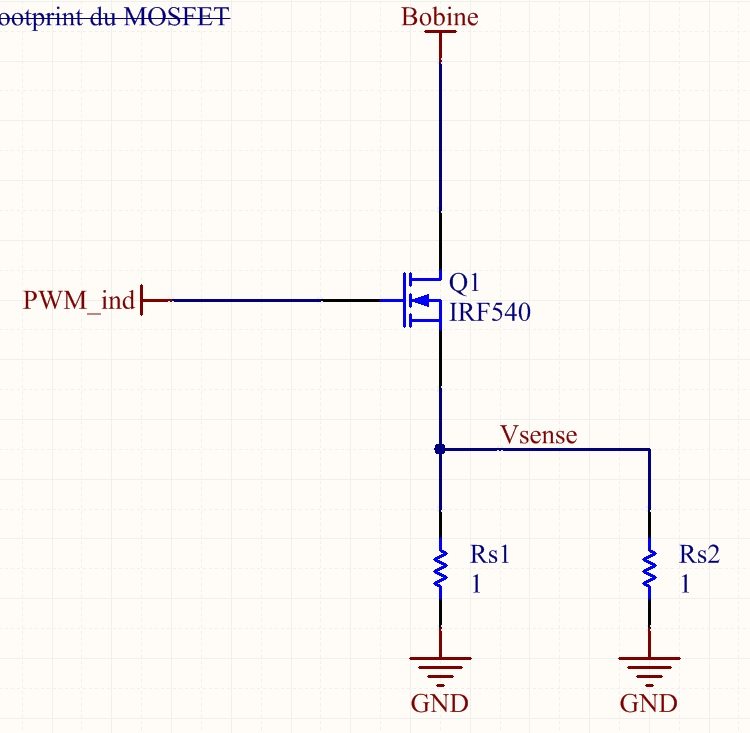
\includegraphics[scale=0.3]{resources/drivemosfet.jpg}
    \caption{Circuit de régulation de la bobine}
  \end{figure}


Pour ajuster la commande du courant, on utilise le trimpot. L'implication de cela est qu'on ne peut pas changer la commande de courant
lorsque le robot va être en train de fonctionner, ainsi on met un peu plus de courant pour générer une FMM plus grande au cas où et aussi il faut que les robot s'enligne directement sur les trésors.
